% Options for packages loaded elsewhere
\PassOptionsToPackage{unicode}{hyperref}
\PassOptionsToPackage{hyphens}{url}
%
\documentclass[
]{article}
\usepackage{amsmath,amssymb}
\usepackage{iftex}
\ifPDFTeX
  \usepackage[T1]{fontenc}
  \usepackage[utf8]{inputenc}
  \usepackage{textcomp} % provide euro and other symbols
\else % if luatex or xetex
  \usepackage{unicode-math} % this also loads fontspec
  \defaultfontfeatures{Scale=MatchLowercase}
  \defaultfontfeatures[\rmfamily]{Ligatures=TeX,Scale=1}
\fi
\usepackage{lmodern}
\ifPDFTeX\else
  % xetex/luatex font selection
\fi
% Use upquote if available, for straight quotes in verbatim environments
\IfFileExists{upquote.sty}{\usepackage{upquote}}{}
\IfFileExists{microtype.sty}{% use microtype if available
  \usepackage[]{microtype}
  \UseMicrotypeSet[protrusion]{basicmath} % disable protrusion for tt fonts
}{}
\makeatletter
\@ifundefined{KOMAClassName}{% if non-KOMA class
  \IfFileExists{parskip.sty}{%
    \usepackage{parskip}
  }{% else
    \setlength{\parindent}{0pt}
    \setlength{\parskip}{6pt plus 2pt minus 1pt}}
}{% if KOMA class
  \KOMAoptions{parskip=half}}
\makeatother
\usepackage{xcolor}
\usepackage[margin=1in]{geometry}
\usepackage{color}
\usepackage{fancyvrb}
\newcommand{\VerbBar}{|}
\newcommand{\VERB}{\Verb[commandchars=\\\{\}]}
\DefineVerbatimEnvironment{Highlighting}{Verbatim}{commandchars=\\\{\}}
% Add ',fontsize=\small' for more characters per line
\usepackage{framed}
\definecolor{shadecolor}{RGB}{248,248,248}
\newenvironment{Shaded}{\begin{snugshade}}{\end{snugshade}}
\newcommand{\AlertTok}[1]{\textcolor[rgb]{0.94,0.16,0.16}{#1}}
\newcommand{\AnnotationTok}[1]{\textcolor[rgb]{0.56,0.35,0.01}{\textbf{\textit{#1}}}}
\newcommand{\AttributeTok}[1]{\textcolor[rgb]{0.13,0.29,0.53}{#1}}
\newcommand{\BaseNTok}[1]{\textcolor[rgb]{0.00,0.00,0.81}{#1}}
\newcommand{\BuiltInTok}[1]{#1}
\newcommand{\CharTok}[1]{\textcolor[rgb]{0.31,0.60,0.02}{#1}}
\newcommand{\CommentTok}[1]{\textcolor[rgb]{0.56,0.35,0.01}{\textit{#1}}}
\newcommand{\CommentVarTok}[1]{\textcolor[rgb]{0.56,0.35,0.01}{\textbf{\textit{#1}}}}
\newcommand{\ConstantTok}[1]{\textcolor[rgb]{0.56,0.35,0.01}{#1}}
\newcommand{\ControlFlowTok}[1]{\textcolor[rgb]{0.13,0.29,0.53}{\textbf{#1}}}
\newcommand{\DataTypeTok}[1]{\textcolor[rgb]{0.13,0.29,0.53}{#1}}
\newcommand{\DecValTok}[1]{\textcolor[rgb]{0.00,0.00,0.81}{#1}}
\newcommand{\DocumentationTok}[1]{\textcolor[rgb]{0.56,0.35,0.01}{\textbf{\textit{#1}}}}
\newcommand{\ErrorTok}[1]{\textcolor[rgb]{0.64,0.00,0.00}{\textbf{#1}}}
\newcommand{\ExtensionTok}[1]{#1}
\newcommand{\FloatTok}[1]{\textcolor[rgb]{0.00,0.00,0.81}{#1}}
\newcommand{\FunctionTok}[1]{\textcolor[rgb]{0.13,0.29,0.53}{\textbf{#1}}}
\newcommand{\ImportTok}[1]{#1}
\newcommand{\InformationTok}[1]{\textcolor[rgb]{0.56,0.35,0.01}{\textbf{\textit{#1}}}}
\newcommand{\KeywordTok}[1]{\textcolor[rgb]{0.13,0.29,0.53}{\textbf{#1}}}
\newcommand{\NormalTok}[1]{#1}
\newcommand{\OperatorTok}[1]{\textcolor[rgb]{0.81,0.36,0.00}{\textbf{#1}}}
\newcommand{\OtherTok}[1]{\textcolor[rgb]{0.56,0.35,0.01}{#1}}
\newcommand{\PreprocessorTok}[1]{\textcolor[rgb]{0.56,0.35,0.01}{\textit{#1}}}
\newcommand{\RegionMarkerTok}[1]{#1}
\newcommand{\SpecialCharTok}[1]{\textcolor[rgb]{0.81,0.36,0.00}{\textbf{#1}}}
\newcommand{\SpecialStringTok}[1]{\textcolor[rgb]{0.31,0.60,0.02}{#1}}
\newcommand{\StringTok}[1]{\textcolor[rgb]{0.31,0.60,0.02}{#1}}
\newcommand{\VariableTok}[1]{\textcolor[rgb]{0.00,0.00,0.00}{#1}}
\newcommand{\VerbatimStringTok}[1]{\textcolor[rgb]{0.31,0.60,0.02}{#1}}
\newcommand{\WarningTok}[1]{\textcolor[rgb]{0.56,0.35,0.01}{\textbf{\textit{#1}}}}
\usepackage{longtable,booktabs,array}
\usepackage{calc} % for calculating minipage widths
% Correct order of tables after \paragraph or \subparagraph
\usepackage{etoolbox}
\makeatletter
\patchcmd\longtable{\par}{\if@noskipsec\mbox{}\fi\par}{}{}
\makeatother
% Allow footnotes in longtable head/foot
\IfFileExists{footnotehyper.sty}{\usepackage{footnotehyper}}{\usepackage{footnote}}
\makesavenoteenv{longtable}
\usepackage{graphicx}
\makeatletter
\def\maxwidth{\ifdim\Gin@nat@width>\linewidth\linewidth\else\Gin@nat@width\fi}
\def\maxheight{\ifdim\Gin@nat@height>\textheight\textheight\else\Gin@nat@height\fi}
\makeatother
% Scale images if necessary, so that they will not overflow the page
% margins by default, and it is still possible to overwrite the defaults
% using explicit options in \includegraphics[width, height, ...]{}
\setkeys{Gin}{width=\maxwidth,height=\maxheight,keepaspectratio}
% Set default figure placement to htbp
\makeatletter
\def\fps@figure{htbp}
\makeatother
\setlength{\emergencystretch}{3em} % prevent overfull lines
\providecommand{\tightlist}{%
  \setlength{\itemsep}{0pt}\setlength{\parskip}{0pt}}
\setcounter{secnumdepth}{-\maxdimen} % remove section numbering
\ifLuaTeX
  \usepackage{selnolig}  % disable illegal ligatures
\fi
\usepackage{bookmark}
\IfFileExists{xurl.sty}{\usepackage{xurl}}{} % add URL line breaks if available
\urlstyle{same}
\hypersetup{
  pdftitle={statistical\_project},
  hidelinks,
  pdfcreator={LaTeX via pandoc}}

\title{statistical\_project}
\author{}
\date{\vspace{-2.5em}2024-05-27}

\begin{document}
\maketitle

\section{Project Introduction}\label{project-introduction}

In this project we aim to study the influence of selected macroeconomics
indicators on the house price index in Colombia. This indicator measure
the evolution through time of the market prices of residential
properties. The idea of the analysis is to present and study the
possible effects of the macroeconomics indicators on the house prices
through the construction of regression models, evaluating their results
and interpreting the models in the context of the data. This will help
understand the main price drivers and could eventually help policy
makers to provide an ecosystem for home affordability.

\section{Dataset Introduction and
Preprocessing}\label{dataset-introduction-and-preprocessing}

The dataset was constructed gathering information from multiple sites:
the Colombian department of statistics (DANE) , the Colombian central
bank (Banco de la República), Google trends queries and the Federal
Reserve Economic Data (FRED). In general, all the visited sites present
the data as a .csv file with tables according to filters related with
the time span of interest. With this we construct a consolidated
database in .csv format with the following variables:

\begin{longtable}[]{@{}
  >{\raggedright\arraybackslash}p{(\columnwidth - 2\tabcolsep) * \real{0.3333}}
  >{\raggedright\arraybackslash}p{(\columnwidth - 2\tabcolsep) * \real{0.6667}}@{}}
\toprule\noalign{}
\begin{minipage}[b]{\linewidth}\raggedright
Variable
\end{minipage} & \begin{minipage}[b]{\linewidth}\raggedright
Description
\end{minipage} \\
\midrule\noalign{}
\endhead
\bottomrule\noalign{}
\endlastfoot
House Price Index & Measure of the average change in the residential
properties price as an index \\
Industrial Inputs Index & Measure of the average changes in the industry
input costs as an index \\
Metals Price Index & Measure of the average price change in metal costs
excluding gold as an index \\
Energy Price Index & Measure of the average price change of energy
including Crude oil, Natural Gas, Coal Price and Propane Indices \\
Shipping Price Index & Measure the average price change of shipping
costs \\
Forex Index & Indicator of the foreign exchange rate of the Colombian
Peso (COP) with respect of the USD \\
Unemployment Rate & Indicator of the percentage of unemployment
population in Colombia \\
Industrial Production Index & Measure of the level of production on
industrial sectors as an index \\
Interest rate & Reference interest rate emited by the colombian central
bank with respect of the others financial institutions \\
Construction Licences Area & Measure the total of squared meters given
for construction licences in Colombia \\
Finished Constructions & Measure of the total constructions that have
been finished in Colombia \\
Google Trends Housing & Google search trends on housing for Colombia \\
\end{longtable}

These variables present real values,and were selected as they have an
initial coherent relation with the housing sector. Initially We present
the import process of the data

\section{Data Uploading}\label{data-uploading}

\begin{Shaded}
\begin{Highlighting}[]
\CommentTok{\#Read the data using the read\_excel function}
\CommentTok{\#Change here for current data path}
\NormalTok{data }\OtherTok{\textless{}{-}} \FunctionTok{read\_excel}\NormalTok{(}\StringTok{"C:/Users/danie/Documents/GitHub/unipd\_sl\_24/data/data.xlsx"}\NormalTok{,}\AttributeTok{sheet =} \StringTok{"dataframe\_col"}\NormalTok{)}
\end{Highlighting}
\end{Shaded}

\section{Data pre-processing and
cleaning}\label{data-pre-processing-and-cleaning}

After have an initial version of the data we proceed with the
pre-processing and cleaning steps. As firs step we change the original
variable names for more appropriate ones. Then we identify the number of
NA values in each one of the columns.

\begin{Shaded}
\begin{Highlighting}[]
\CommentTok{\#change the variables names to have more consistency }
\FunctionTok{colnames}\NormalTok{(data) }\OtherTok{\textless{}{-}} \FunctionTok{c}\NormalTok{(}\StringTok{\textquotesingle{}MY\textquotesingle{}}\NormalTok{,}\StringTok{\textquotesingle{}date\textquotesingle{}}\NormalTok{,}\StringTok{\textquotesingle{}House\_Price\_Index\textquotesingle{}}\NormalTok{,}\StringTok{\textquotesingle{}Industrial\_Inputs\_Index\textquotesingle{}}\NormalTok{,}\StringTok{\textquotesingle{}Metals\_Price\_Index\textquotesingle{}}\NormalTok{,}\StringTok{\textquotesingle{}Energy\_Price\_Index\textquotesingle{}}\NormalTok{,}\StringTok{\textquotesingle{}Shipping\_Price\_Index\textquotesingle{}}\NormalTok{,}\StringTok{\textquotesingle{}Forex\_Index\textquotesingle{}}\NormalTok{,}\StringTok{\textquotesingle{}Unemployment\_Rate\textquotesingle{}}\NormalTok{,}\StringTok{\textquotesingle{}Industrial\_Production\_Index\textquotesingle{}}\NormalTok{,}\StringTok{\textquotesingle{}Interest\_Rate\textquotesingle{}}\NormalTok{,}\StringTok{\textquotesingle{}Construction\_Licences\_Area\textquotesingle{}}\NormalTok{,}\StringTok{\textquotesingle{}Finished\_Constructions\textquotesingle{}}\NormalTok{,}\StringTok{\textquotesingle{}Google\_Trends\_Housing\textquotesingle{}}\NormalTok{) }
\CommentTok{\# Counting NA values in each column}
\NormalTok{na\_counts }\OtherTok{\textless{}{-}} \FunctionTok{apply}\NormalTok{(data, }\DecValTok{2}\NormalTok{, }\ControlFlowTok{function}\NormalTok{(x) }\FunctionTok{sum}\NormalTok{(}\FunctionTok{is.na}\NormalTok{(x)))}
\CommentTok{\# Print the counts of NA values per column}
\FunctionTok{print}\NormalTok{(na\_counts)}
\end{Highlighting}
\end{Shaded}

\begin{verbatim}
##                          MY                        date 
##                           0                           0 
##           House_Price_Index     Industrial_Inputs_Index 
##                           0                           0 
##          Metals_Price_Index          Energy_Price_Index 
##                           0                           0 
##        Shipping_Price_Index                 Forex_Index 
##                           0                           0 
##           Unemployment_Rate Industrial_Production_Index 
##                           0                          12 
##               Interest_Rate  Construction_Licences_Area 
##                           0                          12 
##      Finished_Constructions       Google_Trends_Housing 
##                         158                           0
\end{verbatim}

\begin{Shaded}
\begin{Highlighting}[]
\CommentTok{\# Convert date column to Date type if it\textquotesingle{}s not already}
\NormalTok{data}\SpecialCharTok{$}\NormalTok{date }\OtherTok{\textless{}{-}} \FunctionTok{as.Date}\NormalTok{(data}\SpecialCharTok{$}\NormalTok{date)}
\CommentTok{\# Copy the dataframe to avoid modifying the original one}
\NormalTok{data\_filled }\OtherTok{\textless{}{-}}\NormalTok{ data}
\end{Highlighting}
\end{Shaded}

We realize that the variable Finished\_Constructions requires an
additional pre-processing step because it is recorded by quarters while
the others are registered by months. We propose the following
reconstruction steps for those intermediate months. The idea is to take
the quarterly value and divide it equally among the respective months of
that quarter:

\begin{Shaded}
\begin{Highlighting}[]
\CommentTok{\# Find the indices where the date is at the end of a trimester}
\NormalTok{trimester\_end\_indices }\OtherTok{\textless{}{-}} \FunctionTok{which}\NormalTok{(}\FunctionTok{format}\NormalTok{(data}\SpecialCharTok{$}\NormalTok{date, }\StringTok{"\%m"}\NormalTok{) }\SpecialCharTok{\%in\%} \FunctionTok{c}\NormalTok{(}\StringTok{"03"}\NormalTok{, }\StringTok{"06"}\NormalTok{, }\StringTok{"09"}\NormalTok{, }\StringTok{"12"}\NormalTok{))}
\CommentTok{\# Loop through each trimester end distribute the value}
\ControlFlowTok{for}\NormalTok{ (i }\ControlFlowTok{in}\NormalTok{ trimester\_end\_indices) \{}
  \ControlFlowTok{if}\NormalTok{ (i }\SpecialCharTok{{-}} \DecValTok{2} \SpecialCharTok{\textgreater{}} \DecValTok{0}\NormalTok{) \{}
    \CommentTok{\# Distribute the value to the current month and the previous two months}
\NormalTok{    value\_to\_distribute }\OtherTok{\textless{}{-}}\NormalTok{ data}\SpecialCharTok{$}\NormalTok{Finished\_Constructions[i] }\SpecialCharTok{/} \DecValTok{3}
\NormalTok{    data\_filled}\SpecialCharTok{$}\NormalTok{Finished\_Constructions[i] }\OtherTok{\textless{}{-}}\NormalTok{ value\_to\_distribute}
\NormalTok{    data\_filled}\SpecialCharTok{$}\NormalTok{Finished\_Constructions[i }\SpecialCharTok{{-}} \DecValTok{1}\NormalTok{] }\OtherTok{\textless{}{-}}\NormalTok{ value\_to\_distribute}
\NormalTok{    data\_filled}\SpecialCharTok{$}\NormalTok{Finished\_Constructions[i }\SpecialCharTok{{-}} \DecValTok{2}\NormalTok{] }\OtherTok{\textless{}{-}}\NormalTok{ value\_to\_distribute}
\NormalTok{  \}}
\NormalTok{\}}
\NormalTok{data\_filled}\SpecialCharTok{$}\NormalTok{Finished\_Constructions }\OtherTok{\textless{}{-}} \FunctionTok{na.locf}\NormalTok{(data\_filled}\SpecialCharTok{$}\NormalTok{Finished\_Constructions, }\AttributeTok{na.rm =} \ConstantTok{FALSE}\NormalTok{)}
\end{Highlighting}
\end{Shaded}

\section{Summary stats and final
dataset}\label{summary-stats-and-final-dataset}

We proceed to remove the left rows with NA values eliminating from the
dataset the registers before January 2005. Also, we drop the column MY
also referred to the date in form of MONTH()YEAR(). Finally, we present
an initial summary of the dataset after these transformations. In
particular we see that the House Price Index range present values on
{[}87.35,203.50{]} with an IQR=70.38.

\begin{Shaded}
\begin{Highlighting}[]
\CommentTok{\# Removing rows with any NA values}
\NormalTok{clean\_data }\OtherTok{\textless{}{-}} \FunctionTok{na.omit}\NormalTok{(data\_filled)}
\CommentTok{\# Drop MY column}
\NormalTok{data\_reduced }\OtherTok{\textless{}{-}} \FunctionTok{subset}\NormalTok{(clean\_data, }\AttributeTok{select =} \SpecialCharTok{{-}}\FunctionTok{c}\NormalTok{(MY))}
\end{Highlighting}
\end{Shaded}

\begin{Shaded}
\begin{Highlighting}[]
\NormalTok{summary\_stats }\OtherTok{\textless{}{-}} \FunctionTok{summary}\NormalTok{(data\_reduced[, }\SpecialCharTok{!}\NormalTok{(}\FunctionTok{names}\NormalTok{(data\_reduced) }\SpecialCharTok{\%in\%} \FunctionTok{c}\NormalTok{(}\StringTok{"date"}\NormalTok{))])}
\end{Highlighting}
\end{Shaded}

\begin{longtable}[]{@{}
  >{\raggedright\arraybackslash}p{(\columnwidth - 12\tabcolsep) * \real{0.2188}}
  >{\raggedright\arraybackslash}p{(\columnwidth - 12\tabcolsep) * \real{0.1250}}
  >{\raggedright\arraybackslash}p{(\columnwidth - 12\tabcolsep) * \real{0.1406}}
  >{\raggedright\arraybackslash}p{(\columnwidth - 12\tabcolsep) * \real{0.1250}}
  >{\raggedright\arraybackslash}p{(\columnwidth - 12\tabcolsep) * \real{0.1250}}
  >{\raggedright\arraybackslash}p{(\columnwidth - 12\tabcolsep) * \real{0.1406}}
  >{\raggedright\arraybackslash}p{(\columnwidth - 12\tabcolsep) * \real{0.1250}}@{}}
\toprule\noalign{}
\begin{minipage}[b]{\linewidth}\raggedright
Statistic
\end{minipage} & \begin{minipage}[b]{\linewidth}\raggedright
Min
\end{minipage} & \begin{minipage}[b]{\linewidth}\raggedright
1st Qu.
\end{minipage} & \begin{minipage}[b]{\linewidth}\raggedright
Median
\end{minipage} & \begin{minipage}[b]{\linewidth}\raggedright
Mean
\end{minipage} & \begin{minipage}[b]{\linewidth}\raggedright
3rd Qu.
\end{minipage} & \begin{minipage}[b]{\linewidth}\raggedright
Max
\end{minipage} \\
\midrule\noalign{}
\endhead
\bottomrule\noalign{}
\endlastfoot
House\_Price\_Index & 87.35 & 110.50 & 157.92 & 147.71 & 180.88 &
203.50 \\
Industrial\_Inputs\_Index & 78.67 & 116.02 & 136.26 & 137.78 & 157.65 &
221.14 \\
Metals\_Price\_Index & 74.89 & 121.21 & 143.74 & 145.88 & 172.53 &
234.53 \\
Energy\_Price\_Index & 55.89 & 128.19 & 162.61 & 173.36 & 223.35 &
376.41 \\
Shipping\_Price\_Index & -213.3 & 242.2 & 262.1 & 280.7 & 294.1 &
478.3 \\
Forex\_Index & 0.1712 & 1.1934 & 2.3762 & 2.6762 & 3.2021 & 4.9223 \\
Unemployment\_Rate & 0.07563 & 0.09728 & 0.10970 & 0.11240 & 0.12099 &
0.21972 \\
Industrial\_Production\_Index & 59.82 & 77.94 & 94.44 & 92.87 & 104.85 &
132.46 \\
Interest\_Rate & 0.01750 & 0.03860 & 0.04525 & 0.05551 & 0.06994 &
0.13250 \\
Construction\_Licences\_Area & 233210 & 969559 & 1156424 & 1205587 &
1373585 & 2883878 \\
Finished\_Constructions & 471310 & 775374 & 848663 & 871488 & 962168 &
1335811 \\
Google\_Trends\_Housing & 16.00 & 23.50 & 34.75 & 36.04 & 47.62 &
64.00 \\
\end{longtable}

\section{Exploratory Analysis}\label{exploratory-analysis}

\section{Outliers based on the IQR}\label{outliers-based-on-the-iqr}

As an initial step to better understand the data and its behavior we
find the outliers of each one of the variables using the IQR to select
those points outside the bounds. As a result we found that the variables
that present the most quantity of outliers are the Shipping Price Index,
the Interest Rate and the Unemployment Rate. In addition, we present the
boxplot of these three variables to obtain a clear summary of their
distribution.

\begin{Shaded}
\begin{Highlighting}[]
\CommentTok{\# Function to detect outliers based on IQR}
\NormalTok{detect\_outliers\_single\_var }\OtherTok{\textless{}{-}} \ControlFlowTok{function}\NormalTok{(column) \{}
\NormalTok{  column }\OtherTok{\textless{}{-}} \FunctionTok{na.omit}\NormalTok{(column) }
\NormalTok{  Q1 }\OtherTok{\textless{}{-}} \FunctionTok{quantile}\NormalTok{(column, }\FloatTok{0.25}\NormalTok{, }\AttributeTok{na.rm =} \ConstantTok{TRUE}\NormalTok{)}
\NormalTok{  Q3 }\OtherTok{\textless{}{-}} \FunctionTok{quantile}\NormalTok{(column, }\FloatTok{0.75}\NormalTok{, }\AttributeTok{na.rm =} \ConstantTok{TRUE}\NormalTok{)}
\NormalTok{  IQR }\OtherTok{\textless{}{-}}\NormalTok{ Q3 }\SpecialCharTok{{-}}\NormalTok{ Q1}
\NormalTok{  lower\_bound }\OtherTok{\textless{}{-}}\NormalTok{ Q1 }\SpecialCharTok{{-}} \FloatTok{1.5} \SpecialCharTok{*}\NormalTok{ IQR}
\NormalTok{  upper\_bound }\OtherTok{\textless{}{-}}\NormalTok{ Q3 }\SpecialCharTok{+} \FloatTok{1.5} \SpecialCharTok{*}\NormalTok{ IQR}
\NormalTok{  outliers }\OtherTok{\textless{}{-}}\NormalTok{ column[column }\SpecialCharTok{\textless{}}\NormalTok{ lower\_bound }\SpecialCharTok{|}\NormalTok{ column }\SpecialCharTok{\textgreater{}}\NormalTok{ upper\_bound]}
  \FunctionTok{return}\NormalTok{(outliers)}
\NormalTok{\}}
\CommentTok{\# List to store outliers for each variable}
\NormalTok{outliers\_list }\OtherTok{\textless{}{-}} \FunctionTok{list}\NormalTok{()}
\CommentTok{\# Loop to determine outliers in each column}
\ControlFlowTok{for}\NormalTok{ (var }\ControlFlowTok{in} \FunctionTok{colnames}\NormalTok{(data\_reduced[, }\SpecialCharTok{!}\NormalTok{(}\FunctionTok{names}\NormalTok{(data\_reduced) }\SpecialCharTok{\%in\%} \FunctionTok{c}\NormalTok{(}\StringTok{"date"}\NormalTok{))])) \{}
  \ControlFlowTok{if}\NormalTok{ (}\FunctionTok{is.numeric}\NormalTok{(data[[var]])) \{}
\NormalTok{    outliers\_list[[var]] }\OtherTok{\textless{}{-}} \FunctionTok{detect\_outliers\_single\_var}\NormalTok{(data[[var]])}
\NormalTok{  \}}
\NormalTok{\}}
\FunctionTok{print}\NormalTok{(outliers\_list)}
\end{Highlighting}
\end{Shaded}

\begin{longtable}[]{@{}
  >{\raggedright\arraybackslash}p{(\columnwidth - 2\tabcolsep) * \real{0.2230}}
  >{\raggedright\arraybackslash}p{(\columnwidth - 2\tabcolsep) * \real{0.7770}}@{}}
\toprule\noalign{}
\begin{minipage}[b]{\linewidth}\raggedright
Variable
\end{minipage} & \begin{minipage}[b]{\linewidth}\raggedright
Values
\end{minipage} \\
\midrule\noalign{}
\endhead
\bottomrule\noalign{}
\endlastfoot
House\_Price\_Index & 0 \\
Industrial\_Inputs\_Index & 0 \\
Metals\_Price\_Index & 0 \\
Energy\_Price\_Index & 376.4121 \\
Shipping\_Price\_Index & 374.969, 375.187, 395.268, 446.983, 439.181,
454.407, 468.721, 478.263, 478.216, 471.877, 469.290, 442.591, 456.584,
412.082, 409.599, 443.799, 420.694, 446.214, 462.462 \\
Forex\_Index & 0 \\
Unemployment\_Rate & 0.1725640, 0.2048530, 0.2197200, 0.2035910,
0.2091470, 0.1744270, 0.1629280, 0.1756237 \\
Industrial\_Production\_Index & 0 \\
Interest\_Rate & 0.1141935, 0.1204839, 0.1275000, 0.1275806, 0.1300000,
0.1324194, 0.1325000, 0.1325000 \\
Construction\_Licences\_Area & 2493085, 1988396, 2838778, 2337743,
2331210, 2859035, 2372414, 2052607 \\
Finished\_Constructions & 4007432, 3762696, 1413931 \\
Google\_Trends\_Housing & 0 \\
\end{longtable}

\begin{center}\includegraphics{Project_markdown_v2_files/figure-latex/unnamed-chunk-8-1} \end{center}

The outlier data for the shipping index, unemployment, and interest
rates all relate to the COVID-19 shock. The shipping index crisis in
mid-2022 resulted from the COVID-19 lockdowns (2020-2021), economic
reactivation, and delays in Chinese and Western ports. The unemployment
outliers are due to the initial COVID lockdown in Colombia and the
ensuing economic shock. The high interest rates stem from the Colombian
Central Bank's efforts to control inflation starting in 2021.

\section{Ploting the House Price
Index}\label{ploting-the-house-price-index}

Continuing with the exploratory analysis we plot the variable of House
Price Index to see its behavior through time. It is possible to see a
clear increase tendency starting from the year 2005 until the year 2021,
then a little decay was recorded.

\begin{center}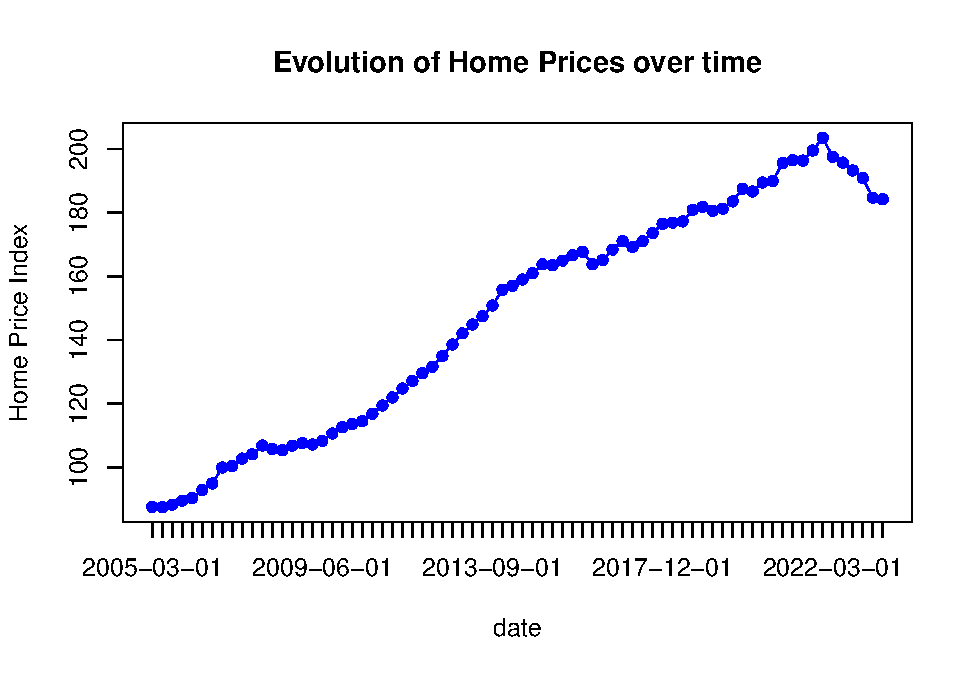
\includegraphics{Project_markdown_v2_files/figure-latex/unnamed-chunk-9-1} \end{center}

\section{Ploting percentual variation of the House Price
Index}\label{ploting-percentual-variation-of-the-house-price-index}

Further useful information can be found in the box plots and histograms
for the percentual variations. We take the 12-period percentual
variation of the variables with the intention of identify patterns and
tendencies in a clear and interpretable way, considering that the
majority of the variables are in index form, and the study of their
changes is fundamental for a complete understanding of their behavior
through time. We start with the House Price Index variable.

In these plots we see that the central value of the percentual
variations is positive, indicating and overall increase in the House
Price Index through time. Also the negatives outliers were expected
because those negatives variations due to the decrease after the 2021.
In the histogram it is possible to see a right skewed behavior, give by
precisely those increments until the 2021.

\begin{Shaded}
\begin{Highlighting}[]
\CommentTok{\# Select subset of variables to difference}
\NormalTok{variables\_to\_calculate }\OtherTok{\textless{}{-}} \FunctionTok{c}\NormalTok{(}\StringTok{"House\_Price\_Index"}\NormalTok{, }\StringTok{"Industrial\_Inputs\_Index"}\NormalTok{, }\StringTok{"Metals\_Price\_Index"}\NormalTok{,}
                            \StringTok{"Energy\_Price\_Index"}\NormalTok{, }\StringTok{"Shipping\_Price\_Index"}\NormalTok{, }\StringTok{"Forex\_Index"}\NormalTok{,}
                            \StringTok{"Industrial\_Production\_Index"}\NormalTok{, }\StringTok{"Construction\_Licences\_Area"}\NormalTok{,}
                            \StringTok{"Finished\_Constructions"}\NormalTok{, }\StringTok{"Google\_Trends\_Housing"}\NormalTok{)}

\CommentTok{\# Create a function to calculate the 12{-}month percentual variation}
\NormalTok{percentual\_variation\_12\_months }\OtherTok{\textless{}{-}} \ControlFlowTok{function}\NormalTok{(x) \{}
  \FunctionTok{return}\NormalTok{((x }\SpecialCharTok{/} \FunctionTok{lag}\NormalTok{(x, }\AttributeTok{n =} \DecValTok{12}\NormalTok{) }\SpecialCharTok{{-}} \DecValTok{1}\NormalTok{))}
\NormalTok{\}}
\NormalTok{lag }\OtherTok{\textless{}{-}} \ControlFlowTok{function}\NormalTok{(x, n) \{}
  \FunctionTok{c}\NormalTok{(}\FunctionTok{rep}\NormalTok{(}\ConstantTok{NA}\NormalTok{, n), }\FunctionTok{head}\NormalTok{(x, }\SpecialCharTok{{-}}\NormalTok{n))}
\NormalTok{\}}
\NormalTok{data\_percentual\_variation }\OtherTok{\textless{}{-}}\NormalTok{ data}
\CommentTok{\# Apply the function to the select variables}
\ControlFlowTok{for}\NormalTok{ (var }\ControlFlowTok{in}\NormalTok{ variables\_to\_calculate) \{}
\NormalTok{  new\_var\_name }\OtherTok{\textless{}{-}} \FunctionTok{paste0}\NormalTok{(}\StringTok{"pct\_var\_"}\NormalTok{, var)}
\NormalTok{  data\_percentual\_variation[[new\_var\_name]] }\OtherTok{\textless{}{-}} \FunctionTok{percentual\_variation\_12\_months}\NormalTok{(data[[var]])}
\NormalTok{\}}
\end{Highlighting}
\end{Shaded}

\begin{center}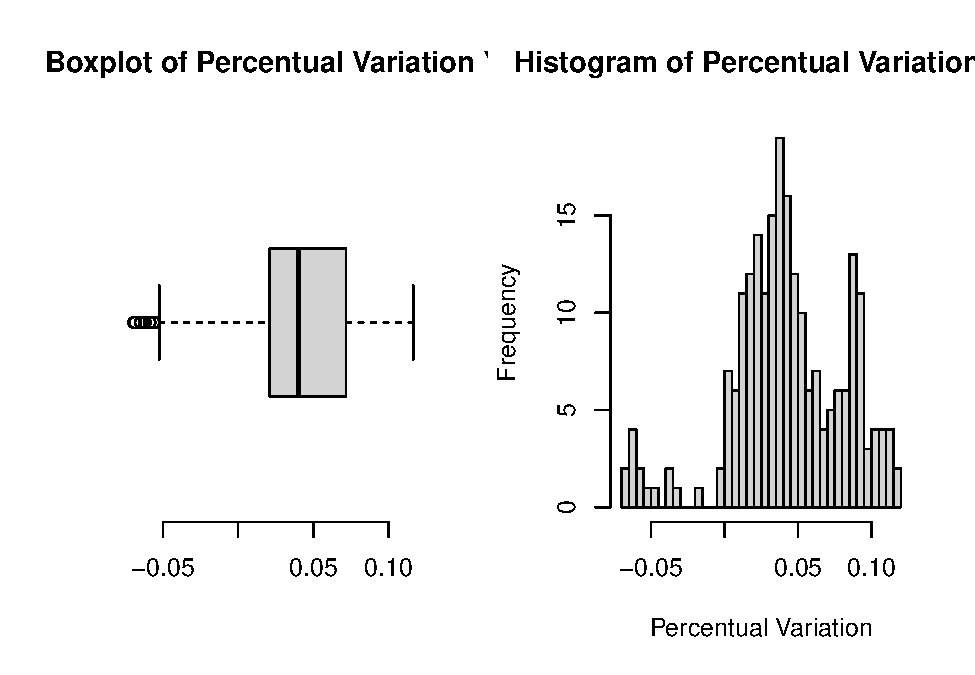
\includegraphics{Project_markdown_v2_files/figure-latex/unnamed-chunk-11-1} \end{center}

We did a similar procedure for the rest of the variables with respect to
their percentual variation. For an easier interpretation we plot the
histograms for the percentual variation of each variable. This plot
shows that the index variables with a high variability in percentual
variation are the shipping index price and the finished constructions.
Also, the index variable that show less variability in the percentual
variation is the one related with the industrial production.

\begin{Shaded}
\begin{Highlighting}[]
\NormalTok{\{}\FunctionTok{par}\NormalTok{(}\AttributeTok{mfrow =} \FunctionTok{c}\NormalTok{(}\DecValTok{3}\NormalTok{,}\DecValTok{4}\NormalTok{ ), }\AttributeTok{mar =} \FunctionTok{c}\NormalTok{(}\DecValTok{2}\NormalTok{, }\DecValTok{2}\NormalTok{, }\DecValTok{2}\NormalTok{, }\DecValTok{2}\NormalTok{) }\SpecialCharTok{+} \FloatTok{0.1}\NormalTok{)}
\NormalTok{data\_percentual\_variation }\OtherTok{\textless{}{-}}\NormalTok{ data\_percentual\_variation[, columns\_to\_select]}
\ControlFlowTok{for}\NormalTok{ (i }\ControlFlowTok{in} \DecValTok{1}\SpecialCharTok{:}\FunctionTok{ncol}\NormalTok{(data\_percentual\_variation)) \{}
  \FunctionTok{hist}\NormalTok{(data\_percentual\_variation[[i]], }
       \AttributeTok{main =} \FunctionTok{substr}\NormalTok{(}\FunctionTok{names}\NormalTok{(data\_percentual\_variation)[i], }\DecValTok{1}\NormalTok{, }\DecValTok{25}\NormalTok{), }\CommentTok{\# Shorten title if necessary}
       \AttributeTok{xlab =} \FunctionTok{names}\NormalTok{(data\_percentual\_variation)[i], }
       \AttributeTok{col =} \StringTok{"blue"}\NormalTok{, }
       \AttributeTok{border =} \StringTok{"black"}\NormalTok{)}
\NormalTok{\}}
\NormalTok{\}}
\end{Highlighting}
\end{Shaded}

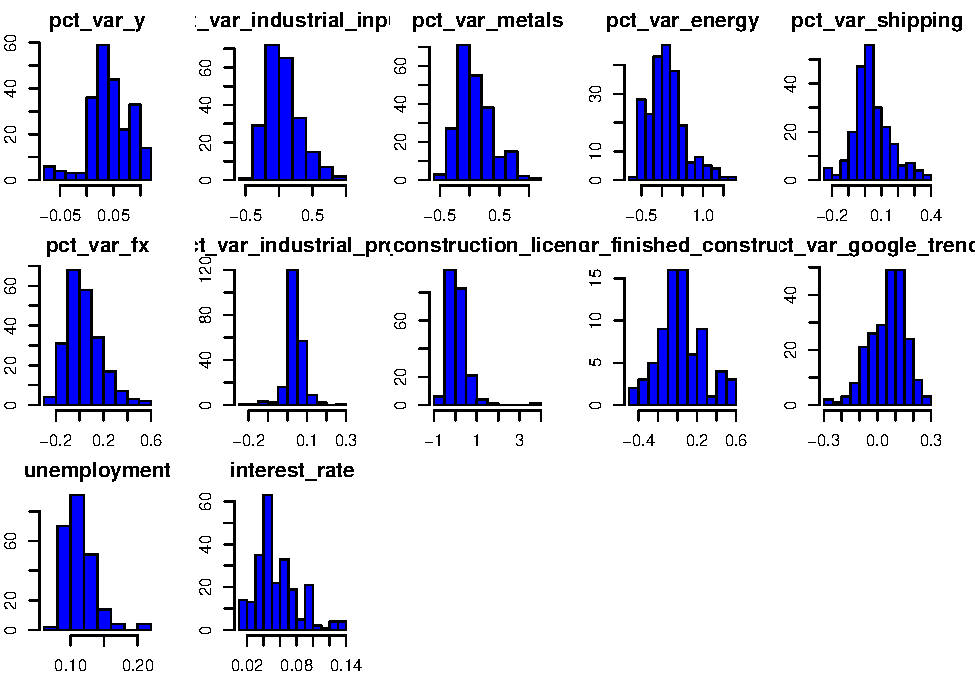
\includegraphics{Project_markdown_v2_files/figure-latex/unnamed-chunk-12-1.pdf}

We plot these four variables to see its evolution through time. It is
possible to see that the industrial production Index and the Shipping
price Index have an increase tendency, with some peaks as for example
the negative peak related with the COVID pandemic for the Industrial
Production Index on the 2020. In another hand, the Finished
Constructions have a less defined behavior over time.

\begin{center}\includegraphics{Project_markdown_v2_files/figure-latex/unnamed-chunk-14-1} \end{center}

\section{Log-transformation}\label{log-transformation}

We apply a log transformation with the intention of scaling the data as
some variables are index that change over time and others area real
values with wider range. Our goal is to reduce the variability of the
data, compressing the scale and helping to linearize those relationships
between the variables for the interpretability of the results in the
subsequent models. We apply log transformation to all variables except
those that are already percentages: the Unemployment Rate and the
Interest Rate.

\begin{Shaded}
\begin{Highlighting}[]
\CommentTok{\#Log transformation of the variables}
\NormalTok{variables\_to\_log }\OtherTok{\textless{}{-}} \FunctionTok{c}\NormalTok{(}\StringTok{"House\_Price\_Index"}\NormalTok{, }\StringTok{"Industrial\_Inputs\_Index"}\NormalTok{, }\StringTok{"Metals\_Price\_Index"}\NormalTok{,}
                      \StringTok{"Energy\_Price\_Index"}\NormalTok{, }\StringTok{"Shipping\_Price\_Index"}\NormalTok{, }\StringTok{"Forex\_Index"}\NormalTok{,}
                      \StringTok{"Industrial\_Production\_Index"}\NormalTok{, }\StringTok{"Construction\_Licences\_Area"}\NormalTok{,}
                      \StringTok{"Finished\_Constructions"}\NormalTok{, }\StringTok{"Google\_Trends\_Housing"}\NormalTok{)}


\ControlFlowTok{for}\NormalTok{ (var }\ControlFlowTok{in}\NormalTok{ variables\_to\_log) \{}
\NormalTok{  log\_var\_name }\OtherTok{\textless{}{-}} \FunctionTok{paste0}\NormalTok{(var, }\StringTok{"\_log"}\NormalTok{)}
\NormalTok{  data\_reduced[[log\_var\_name]] }\OtherTok{\textless{}{-}} \FunctionTok{log}\NormalTok{(data\_reduced[[var]])}
\NormalTok{\}}

\CommentTok{\# Subset the dataframe}
\NormalTok{selected\_columns }\OtherTok{\textless{}{-}} \FunctionTok{c}\NormalTok{(}\FunctionTok{paste0}\NormalTok{(variables\_to\_log, }\StringTok{"\_log"}\NormalTok{), }\StringTok{"Unemployment\_Rate"}\NormalTok{, }\StringTok{"Interest\_Rate"}\NormalTok{)}
\NormalTok{data\_final }\OtherTok{\textless{}{-}}\NormalTok{ data\_reduced[, selected\_columns]}
\end{Highlighting}
\end{Shaded}

\section{Variable Correlation}\label{variable-correlation}

Now we present the correlation between the variables of the dataset in
order to understand the strength of their relation. We present the
correlation matrix obtained. From the results we see a strong positive
relationship between the House Price Index and the Google Trend and
Industrial Production one,a more moderate correlation with the shipping
Price and the Forex Index. While the weaker relationships are found with
the Energy Price index and the Unemployment Rate.For the others
variables, we found a high positive correlation between the metal price
index and the industrial inputs.

\begin{Shaded}
\begin{Highlighting}[]
\CommentTok{\# Plot the correlation matrix }

\NormalTok{\{}\FunctionTok{par}\NormalTok{(}\AttributeTok{mar =} \FunctionTok{c}\NormalTok{(}\DecValTok{7}\NormalTok{, }\DecValTok{7}\NormalTok{, }\DecValTok{7}\NormalTok{, }\DecValTok{2}\NormalTok{) }\SpecialCharTok{+} \FloatTok{0.1}\NormalTok{)}
\NormalTok{cor\_matrix}\OtherTok{\textless{}{-}}\NormalTok{correl\_matrix}
\FunctionTok{image}\NormalTok{(}\DecValTok{1}\SpecialCharTok{:}\FunctionTok{ncol}\NormalTok{(cor\_matrix), }\DecValTok{1}\SpecialCharTok{:}\FunctionTok{nrow}\NormalTok{(cor\_matrix), }\FunctionTok{t}\NormalTok{(cor\_matrix)[, }\FunctionTok{ncol}\NormalTok{(cor\_matrix)}\SpecialCharTok{:}\DecValTok{1}\NormalTok{], }
      \AttributeTok{axes =} \ConstantTok{FALSE}\NormalTok{, }\AttributeTok{xlab =} \StringTok{""}\NormalTok{, }\AttributeTok{ylab =} \StringTok{""}\NormalTok{, }\AttributeTok{col =} \FunctionTok{colorRampPalette}\NormalTok{(}\FunctionTok{c}\NormalTok{(}\StringTok{"red"}\NormalTok{, }\StringTok{"white"}\NormalTok{, }\StringTok{"blue"}\NormalTok{))(}\DecValTok{20}\NormalTok{))}

\CommentTok{\# Add axis labels }
\FunctionTok{axis}\NormalTok{(}\DecValTok{3}\NormalTok{, }\AttributeTok{at =} \DecValTok{1}\SpecialCharTok{:}\FunctionTok{ncol}\NormalTok{(cor\_matrix), }\AttributeTok{labels =} \FunctionTok{colnames}\NormalTok{(cor\_matrix), }\AttributeTok{las =} \DecValTok{2}\NormalTok{, }\AttributeTok{cex.axis =} \FloatTok{0.7}\NormalTok{)}
\FunctionTok{axis}\NormalTok{(}\DecValTok{2}\NormalTok{, }\AttributeTok{at =} \DecValTok{1}\SpecialCharTok{:}\FunctionTok{nrow}\NormalTok{(cor\_matrix), }\AttributeTok{labels =} \FunctionTok{rev}\NormalTok{(}\FunctionTok{rownames}\NormalTok{(cor\_matrix)), }\AttributeTok{las =} \DecValTok{2}\NormalTok{, }\AttributeTok{cex.axis =} \FloatTok{0.7}\NormalTok{)}

\CommentTok{\#correlation coefficients}
\ControlFlowTok{for}\NormalTok{ (i }\ControlFlowTok{in} \DecValTok{1}\SpecialCharTok{:}\FunctionTok{ncol}\NormalTok{(cor\_matrix)) \{}
  \ControlFlowTok{for}\NormalTok{ (j }\ControlFlowTok{in} \DecValTok{1}\SpecialCharTok{:}\FunctionTok{nrow}\NormalTok{(cor\_matrix)) \{}
    \FunctionTok{text}\NormalTok{(i, }\FunctionTok{nrow}\NormalTok{(cor\_matrix) }\SpecialCharTok{{-}}\NormalTok{ j }\SpecialCharTok{+} \DecValTok{1}\NormalTok{, }\FunctionTok{round}\NormalTok{(cor\_matrix[i, j], }\DecValTok{2}\NormalTok{), }\AttributeTok{cex =} \FloatTok{0.7}\NormalTok{)}
\NormalTok{  \}}
\NormalTok{\}\}}
\end{Highlighting}
\end{Shaded}

\includegraphics{Project_markdown_v2_files/figure-latex/unnamed-chunk-18-1.pdf}

\section{Multicolinearity Check}\label{multicolinearity-check}

Now present a multicollinearity test in top of the results related with
the correlation of the variables in relation with the dependent variable
of House Price Index. We first calculate the VIF for each predictor
variable. We found that some variables like Shipping, Industrial
Production Index, Metals Price Index and Industrial Inputs present a
high VIF.

\begin{verbatim}
##     Industrial_Inputs_Index_log          Metals_Price_Index_log 
##                      232.372573                      237.983290 
##          Energy_Price_Index_log        Shipping_Price_Index_log 
##                        6.176604                       12.188511 
##                 Forex_Index_log Industrial_Production_Index_log 
##                       10.143101                       17.856757 
##  Construction_Licences_Area_log      Finished_Constructions_log 
##                        1.807047                        2.148915 
##       Google_Trends_Housing_log               Unemployment_Rate 
##                        8.171922                        4.286584 
##                   Interest_Rate 
##                        1.982209
\end{verbatim}

At this point we consider to remove the Metals Price Index as they show
a strong correlation with Industrial Inputs, they both have a similar
behavior and at the end the metal sector is considered on the Industrial
Inputs Index. After this reduction we re run the VIF test. There are
some variables that show high VIF, but due to the economic literature we
decide to keep going with them. Later we will perform variable selection
through different approaches and eventually the multicolinearity here
present will be corrected.

\begin{verbatim}
##     Industrial_Inputs_Index_log          Energy_Price_Index_log 
##                        3.479427                        6.171898 
##        Shipping_Price_Index_log                 Forex_Index_log 
##                       11.954143                       10.092636 
## Industrial_Production_Index_log  Construction_Licences_Area_log 
##                       14.752680                        1.698461 
##      Finished_Constructions_log       Google_Trends_Housing_log 
##                        2.102236                        8.037613 
##               Unemployment_Rate                   Interest_Rate 
##                        3.673045                        1.900964
\end{verbatim}

\section{Train Test Split}\label{train-test-split}

Before proceed with the linear models we apply a train test split in
order to have a test set to compare the performance in a fair way
between the data. For this we implement the following steps, considering
that our train set will be 80\% of the data:

\begin{Shaded}
\begin{Highlighting}[]
\FunctionTok{set.seed}\NormalTok{(}\DecValTok{123}\NormalTok{)  }
\CommentTok{\# sample index for training data}
\NormalTok{trainIndex }\OtherTok{\textless{}{-}} \FunctionTok{sample}\NormalTok{(}\FunctionTok{seq\_len}\NormalTok{(}\FunctionTok{nrow}\NormalTok{(data\_final)), }\AttributeTok{size =} \FloatTok{0.8} \SpecialCharTok{*} \FunctionTok{nrow}\NormalTok{(data\_final))}
\CommentTok{\# Split the data into training and testing sets}
\NormalTok{data\_train }\OtherTok{\textless{}{-}}\NormalTok{ data\_final[trainIndex, ]}
\NormalTok{data\_test }\OtherTok{\textless{}{-}}\NormalTok{ data\_final[}\SpecialCharTok{{-}}\NormalTok{trainIndex, ]}

\NormalTok{X\_train }\OtherTok{\textless{}{-}} \FunctionTok{model.matrix}\NormalTok{(House\_Price\_Index\_log }\SpecialCharTok{\textasciitilde{}}\NormalTok{ ., }\AttributeTok{data =}\NormalTok{ data\_train)[, }\SpecialCharTok{{-}}\DecValTok{1}\NormalTok{] }
\NormalTok{y\_train }\OtherTok{\textless{}{-}}\NormalTok{ data\_train}\SpecialCharTok{$}\NormalTok{House\_Price\_Index\_log}
\NormalTok{X\_test }\OtherTok{\textless{}{-}} \FunctionTok{model.matrix}\NormalTok{(House\_Price\_Index\_log }\SpecialCharTok{\textasciitilde{}}\NormalTok{ ., }\AttributeTok{data =}\NormalTok{ data\_test)[, }\SpecialCharTok{{-}}\DecValTok{1}\NormalTok{] }
\NormalTok{y\_test }\OtherTok{\textless{}{-}}\NormalTok{ data\_test}\SpecialCharTok{$}\NormalTok{House\_Price\_Index\_log}
\end{Highlighting}
\end{Shaded}

\section{Modelling the data}\label{modelling-the-data}

\#Initial full linear model We start with a simple regression model for
the data, remember that this process will be executed with the variables
after the log normalization. In this first iteration we consider all the
explanatory variables.

\begin{Shaded}
\begin{Highlighting}[]
\CommentTok{\# OLS 1 Log{-}Log{-}{-}{-}{-}{-}{-}{-}{-}{-}{-}{-}{-}{-}{-}{-}{-}{-}}
\CommentTok{\# Perform linear regression}
\NormalTok{model }\OtherTok{\textless{}{-}} \FunctionTok{lm}\NormalTok{(House\_Price\_Index\_log }\SpecialCharTok{\textasciitilde{}}\NormalTok{ ., }\AttributeTok{data =}\NormalTok{ data\_train)  }
\FunctionTok{summary}\NormalTok{(model)}
\end{Highlighting}
\end{Shaded}

\begin{verbatim}
## 
## Call:
## lm(formula = House_Price_Index_log ~ ., data = data_train)
## 
## Residuals:
##       Min        1Q    Median        3Q       Max 
## -0.088670 -0.019984  0.001724  0.019942  0.092810 
## 
## Coefficients:
##                                 Estimate Std. Error t value Pr(>|t|)    
## (Intercept)                      0.79395    0.31588   2.513 0.012898 *  
## Industrial_Inputs_Index_log     -0.03332    0.01994  -1.671 0.096516 .  
## Energy_Price_Index_log           0.01794    0.01808   0.992 0.322477    
## Shipping_Price_Index_log         0.07971    0.04815   1.656 0.099658 .  
## Forex_Index_log                 -0.07641    0.02797  -2.732 0.006973 ** 
## Industrial_Production_Index_log  0.80968    0.05384  15.040  < 2e-16 ***
## Construction_Licences_Area_log  -0.02418    0.01060  -2.282 0.023760 *  
## Finished_Constructions_log      -0.01036    0.01879  -0.551 0.582041    
## Google_Trends_Housing_log        0.32995    0.01873  17.620  < 2e-16 ***
## Unemployment_Rate                0.76654    0.23145   3.312 0.001134 ** 
## Interest_Rate                   -0.47954    0.12981  -3.694 0.000298 ***
## ---
## Signif. codes:  0 '***' 0.001 '**' 0.01 '*' 0.05 '.' 0.1 ' ' 1
## 
## Residual standard error: 0.03321 on 168 degrees of freedom
## Multiple R-squared:  0.9846, Adjusted R-squared:  0.9837 
## F-statistic:  1075 on 10 and 168 DF,  p-value: < 2.2e-16
\end{verbatim}

In this first model we see a high R-squared, this mean that the model is
powerful in terms of explain the variability in the House Price Index,
but the model is no completely satisfactory as it includes several
predictors without statistical significance, and other with different
degree of significance as Industrial Production Index, Google Trends
Housing and Interest Rate. This can be explain because the R-squared
statistic will always increase when more variables are added to the
model. We proceed to plot the the results for the fitted results and the
QQ-plot of the residuals:

\includegraphics{Project_markdown_v2_files/figure-latex/unnamed-chunk-23-1.pdf}

After having the model we fit it to evaluate its performance. First we
determine the MSE which has a value of 0.00269 suggesting the the
predictions are close to the actual values, this could be observed in
the plot of the predicted vs the actual values which presents an
approximately 45° degrees line.

\begin{verbatim}
## [1] 0.00186722
\end{verbatim}

\includegraphics{Project_markdown_v2_files/figure-latex/unnamed-chunk-24-1.pdf}

\section{Model dropping variables according to their
significance}\label{model-dropping-variables-according-to-their-significance}

After the first iteration we consider the process of eliminating
variables based on its significance to the model. The first variable
that we consider to discard is the Energy Price Index, for this we
proceed with an ANOVA F-test for the comparison of regression models. As
the obtained value is 0.1328 is greater than 0.05 the Energy Price Index
is not a significant predictor in the presence of the other variables.
With this we remove it

\begin{verbatim}
## 
## Call:
## lm(formula = House_Price_Index_log ~ ., data = data_train)
## 
## Residuals:
##       Min        1Q    Median        3Q       Max 
## -0.088670 -0.019984  0.001724  0.019942  0.092810 
## 
## Coefficients:
##                                 Estimate Std. Error t value Pr(>|t|)    
## (Intercept)                      0.79395    0.31588   2.513 0.012898 *  
## Industrial_Inputs_Index_log     -0.03332    0.01994  -1.671 0.096516 .  
## Energy_Price_Index_log           0.01794    0.01808   0.992 0.322477    
## Shipping_Price_Index_log         0.07971    0.04815   1.656 0.099658 .  
## Forex_Index_log                 -0.07641    0.02797  -2.732 0.006973 ** 
## Industrial_Production_Index_log  0.80968    0.05384  15.040  < 2e-16 ***
## Construction_Licences_Area_log  -0.02418    0.01060  -2.282 0.023760 *  
## Finished_Constructions_log      -0.01036    0.01879  -0.551 0.582041    
## Google_Trends_Housing_log        0.32995    0.01873  17.620  < 2e-16 ***
## Unemployment_Rate                0.76654    0.23145   3.312 0.001134 ** 
## Interest_Rate                   -0.47954    0.12981  -3.694 0.000298 ***
## ---
## Signif. codes:  0 '***' 0.001 '**' 0.01 '*' 0.05 '.' 0.1 ' ' 1
## 
## Residual standard error: 0.03321 on 168 degrees of freedom
## Multiple R-squared:  0.9846, Adjusted R-squared:  0.9837 
## F-statistic:  1075 on 10 and 168 DF,  p-value: < 2.2e-16
\end{verbatim}

\begin{verbatim}
## Analysis of Variance Table
## 
## Model 1: House_Price_Index_log ~ Industrial_Inputs_Index_log + Shipping_Price_Index_log + 
##     Forex_Index_log + Industrial_Production_Index_log + Construction_Licences_Area_log + 
##     Finished_Constructions_log + Google_Trends_Housing_log + 
##     Unemployment_Rate + Interest_Rate
## Model 2: House_Price_Index_log ~ Industrial_Inputs_Index_log + Energy_Price_Index_log + 
##     Shipping_Price_Index_log + Forex_Index_log + Industrial_Production_Index_log + 
##     Construction_Licences_Area_log + Finished_Constructions_log + 
##     Google_Trends_Housing_log + Unemployment_Rate + Interest_Rate
##   Res.Df     RSS Df Sum of Sq      F Pr(>F)
## 1    169 0.18643                           
## 2    168 0.18534  1 0.0010863 0.9847 0.3225
\end{verbatim}

We observe again the significance of the variables, and the next no
significant variables that we decide to drop were Industrial Inputs
Index, Finished Constructions. All of this after eliminating step by
step each one following the previous procedure with the ANOVA F-test
until all the predictors show statistical evidence of having coefficient
different from 0.

\begin{Shaded}
\begin{Highlighting}[]
\CommentTok{\#Process of Variable dropping according to ther significance}

\CommentTok{\# Energy does not improve model}
\FunctionTok{summary}\NormalTok{(red.mod)}
\NormalTok{red.mod2 }\OtherTok{\textless{}{-}} \FunctionTok{update}\NormalTok{(red.mod, . }\SpecialCharTok{\textasciitilde{}}\NormalTok{ . }\SpecialCharTok{{-}}\NormalTok{Industrial\_Inputs\_Index\_log)}
\FunctionTok{anova}\NormalTok{(red.mod, red.mod2)}
\CommentTok{\# Can safely remove industrial inputs log}
\FunctionTok{summary}\NormalTok{(red.mod2)}

\CommentTok{\# Remove finished\_constructions\_log }
\NormalTok{red.mod3 }\OtherTok{\textless{}{-}} \FunctionTok{update}\NormalTok{(red.mod2, . }\SpecialCharTok{\textasciitilde{}}\NormalTok{ . }\SpecialCharTok{{-}}\NormalTok{Finished\_Constructions\_log)}
\FunctionTok{anova}\NormalTok{(red.mod2, red.mod3)}
\CommentTok{\# Can safely remove finished constructions (but makes no sense)}
\FunctionTok{summary}\NormalTok{(red.mod3)}
\end{Highlighting}
\end{Shaded}

\begin{verbatim}
## 
## Call:
## lm(formula = House_Price_Index_log ~ Shipping_Price_Index_log + 
##     Forex_Index_log + Industrial_Production_Index_log + Construction_Licences_Area_log + 
##     Google_Trends_Housing_log + Unemployment_Rate + Interest_Rate, 
##     data = data_train)
## 
## Residuals:
##       Min        1Q    Median        3Q       Max 
## -0.094159 -0.021217 -0.000685  0.021851  0.090717 
## 
## Coefficients:
##                                 Estimate Std. Error t value Pr(>|t|)    
## (Intercept)                      0.64293    0.16678   3.855 0.000164 ***
## Shipping_Price_Index_log         0.09061    0.02805   3.231 0.001481 ** 
## Forex_Index_log                 -0.06931    0.01801  -3.849 0.000167 ***
## Industrial_Production_Index_log  0.77431    0.04870  15.901  < 2e-16 ***
## Construction_Licences_Area_log  -0.02490    0.01038  -2.399 0.017496 *  
## Google_Trends_Housing_log        0.33191    0.01750  18.968  < 2e-16 ***
## Unemployment_Rate                0.61628    0.18912   3.259 0.001351 ** 
## Interest_Rate                   -0.46996    0.12859  -3.655 0.000342 ***
## ---
## Signif. codes:  0 '***' 0.001 '**' 0.01 '*' 0.05 '.' 0.1 ' ' 1
## 
## Residual standard error: 0.03321 on 171 degrees of freedom
## Multiple R-squared:  0.9843, Adjusted R-squared:  0.9837 
## F-statistic:  1535 on 7 and 171 DF,  p-value: < 2.2e-16
\end{verbatim}

\includegraphics{Project_markdown_v2_files/figure-latex/unnamed-chunk-28-1.pdf}
The final reduced model continue to show a high R-squared, while the
QQ-Plot shows similar points outside the reference line. At this point
even the fact that now all the variables are statistically significant,
the model appears to has more or less the same explanatory power due to
the residuals behavior.

\begin{verbatim}
## [1] 0.001830836
\end{verbatim}

\includegraphics{Project_markdown_v2_files/figure-latex/unnamed-chunk-29-1.pdf}

\section{Model with lagged variable}\label{model-with-lagged-variable}

As a following step we implement a procedure to consider a lag version
of the House Price Index, this due to the possible influence of lagged
affects, in terms of the intuition that the actual house price index
will not be determined by the current explanatory variables, but by the
explanatory variables of the previous period. Research conducted by
Iacoviello, Matteo (2004) suggests that the house prices can be modeled
with a VAR approach, which considers lags of both the dependent variable
and the covariates. We include so far only the dependent variable due to
the modelling approach in this written (Linear Regression Analysis).
Unemployment Rate was discarded because its coefficient showed no
evidence of being different from zero, and via the ANOVA analysis it
could be concluded that it was safe to discard it.

\begin{Shaded}
\begin{Highlighting}[]
\CommentTok{\# Using a a lag version of the House Price Index}

\NormalTok{data\_final\_with\_lag}\OtherTok{\textless{}{-}}\NormalTok{ data\_final}

\NormalTok{data\_final\_with\_lag}\SpecialCharTok{$}\NormalTok{House\_Price\_Index\_log\_lag1 }\OtherTok{\textless{}{-}} \FunctionTok{c}\NormalTok{(}\ConstantTok{NA}\NormalTok{, }\FunctionTok{head}\NormalTok{(data\_final}\SpecialCharTok{$}\NormalTok{House\_Price\_Index\_log, }\SpecialCharTok{{-}}\DecValTok{1}\NormalTok{))}

\NormalTok{data\_final\_with\_lag }\OtherTok{\textless{}{-}} \FunctionTok{na.omit}\NormalTok{(data\_final\_with\_lag)}
\end{Highlighting}
\end{Shaded}

\begin{Shaded}
\begin{Highlighting}[]
\CommentTok{\# Set the seed for reproducibility}
\FunctionTok{set.seed}\NormalTok{(}\DecValTok{123}\NormalTok{)}

\NormalTok{trainIndex\_lag }\OtherTok{\textless{}{-}} \FunctionTok{sample}\NormalTok{(}\FunctionTok{seq\_len}\NormalTok{(}\FunctionTok{nrow}\NormalTok{(data\_final\_with\_lag)), }\AttributeTok{size =} \FloatTok{0.8} \SpecialCharTok{*} \FunctionTok{nrow}\NormalTok{(data\_final\_with\_lag))}

\CommentTok{\# Split the data into training and testing sets}
\NormalTok{data\_train\_lag }\OtherTok{\textless{}{-}}\NormalTok{ data\_final\_with\_lag[trainIndex\_lag, ]}
\NormalTok{data\_test\_lag }\OtherTok{\textless{}{-}}\NormalTok{ data\_final\_with\_lag[}\SpecialCharTok{{-}}\NormalTok{trainIndex\_lag, ]}


\NormalTok{X\_train\_lag }\OtherTok{\textless{}{-}} \FunctionTok{model.matrix}\NormalTok{(House\_Price\_Index\_log }\SpecialCharTok{\textasciitilde{}}\NormalTok{ ., }\AttributeTok{data =}\NormalTok{ data\_train\_lag)[, }\SpecialCharTok{{-}}\DecValTok{1}\NormalTok{] }
\NormalTok{y\_train\_lag }\OtherTok{\textless{}{-}}\NormalTok{ data\_train\_lag}\SpecialCharTok{$}\NormalTok{House\_Price\_Index\_log}


\NormalTok{X\_test\_lag }\OtherTok{\textless{}{-}} \FunctionTok{model.matrix}\NormalTok{(House\_Price\_Index\_log }\SpecialCharTok{\textasciitilde{}}\NormalTok{ ., }\AttributeTok{data =}\NormalTok{ data\_test\_lag)[, }\SpecialCharTok{{-}}\DecValTok{1}\NormalTok{]  }
\NormalTok{y\_test\_lag }\OtherTok{\textless{}{-}}\NormalTok{ data\_test\_lag}\SpecialCharTok{$}\NormalTok{House\_Price\_Index\_log}
\end{Highlighting}
\end{Shaded}

\begin{Shaded}
\begin{Highlighting}[]
\NormalTok{model\_lag }\OtherTok{\textless{}{-}} \FunctionTok{lm}\NormalTok{(House\_Price\_Index\_log }\SpecialCharTok{\textasciitilde{}}\NormalTok{ House\_Price\_Index\_log\_lag1 }\SpecialCharTok{+}\NormalTok{Forex\_Index\_log}\SpecialCharTok{+}\NormalTok{Industrial\_Production\_Index\_log}\SpecialCharTok{+}\NormalTok{Construction\_Licences\_Area\_log}\SpecialCharTok{+}\NormalTok{Google\_Trends\_Housing\_log}\SpecialCharTok{+}\NormalTok{Interest\_Rate, }\AttributeTok{data =}\NormalTok{ data\_train\_lag)}

\CommentTok{\# Summarize the model}
\FunctionTok{summary}\NormalTok{(model\_lag)}
\end{Highlighting}
\end{Shaded}

\begin{verbatim}
## 
## Call:
## lm(formula = House_Price_Index_log ~ House_Price_Index_log_lag1 + 
##     Forex_Index_log + Industrial_Production_Index_log + Construction_Licences_Area_log + 
##     Google_Trends_Housing_log + Interest_Rate, data = data_train_lag)
## 
## Residuals:
##       Min        1Q    Median        3Q       Max 
## -0.011794 -0.002766  0.000083  0.003037  0.015861 
## 
## Coefficients:
##                                  Estimate Std. Error t value Pr(>|t|)    
## (Intercept)                      0.110388   0.023991   4.601 8.15e-06 ***
## House_Price_Index_log_lag1       0.963768   0.009419 102.321  < 2e-16 ***
## Forex_Index_log                 -0.009077   0.002165  -4.193 4.40e-05 ***
## Industrial_Production_Index_log  0.037624   0.008286   4.540 1.06e-05 ***
## Construction_Licences_Area_log  -0.003591   0.001491  -2.408   0.0171 *  
## Google_Trends_Housing_log        0.008054   0.004049   1.989   0.0483 *  
## Interest_Rate                   -0.079478   0.017003  -4.674 5.96e-06 ***
## ---
## Signif. codes:  0 '***' 0.001 '**' 0.01 '*' 0.05 '.' 0.1 ' ' 1
## 
## Residual standard error: 0.00486 on 171 degrees of freedom
## Multiple R-squared:  0.9997, Adjusted R-squared:  0.9996 
## F-statistic: 8.361e+04 on 6 and 171 DF,  p-value: < 2.2e-16
\end{verbatim}

After include the lagged effect we consider the reduced model showing a
high R-squared. Then we proceed to show the histogram of the residuals
and their QQ plot. From the QQ-plot it is possible to see that now the
residuals show a even strong normal behavior

\includegraphics{Project_markdown_v2_files/figure-latex/unnamed-chunk-33-1.pdf}

Now, it is possible to see that the fit of the predictions and actual
values is more correct, in terms that it follows almost a a perfect
straight line.

\begin{verbatim}
## [1] 2.317564e-05
\end{verbatim}

\includegraphics{Project_markdown_v2_files/figure-latex/unnamed-chunk-34-1.pdf}

\section{Forward AIC Selection model}\label{forward-aic-selection-model}

We Implement the forward selection based on the AIC for a family of
models. The AIC approach allows a model comparison with the aim to find
a good balance between model fit and complexity. The process of forward
selection starts with no predictors (just with the bias) and adds one by
one each of the covariates from the pre-cured dataframe. We could see
variables with no statistical evidence of significance using this
approach. This happens because via the AIC forward selection method is
possible to obtain non-significant coefficients for a given set of
variables but their inclusion minimizes the AIC.

\begin{Shaded}
\begin{Highlighting}[]
\CommentTok{\# Forward AIC Stepwise selection{-}{-}{-}{-}{-}{-}{-}{-}{-}{-}{-}{-}{-}}

\CommentTok{\# Fit the null model (intercept only)}
\NormalTok{null\_model }\OtherTok{\textless{}{-}} \FunctionTok{lm}\NormalTok{(House\_Price\_Index\_log }\SpecialCharTok{\textasciitilde{}} \DecValTok{1}\NormalTok{, }\AttributeTok{data =}\NormalTok{ data\_train)}

\CommentTok{\# Specify the full model with all potential predictors}
\NormalTok{full\_model }\OtherTok{\textless{}{-}} \FunctionTok{lm}\NormalTok{(House\_Price\_Index\_log }\SpecialCharTok{\textasciitilde{}}\NormalTok{ Industrial\_Inputs\_Index\_log }\SpecialCharTok{+}\NormalTok{ Shipping\_Price\_Index\_log }\SpecialCharTok{+}\NormalTok{ Forex\_Index\_log }\SpecialCharTok{+}\NormalTok{ Industrial\_Production\_Index\_log }\SpecialCharTok{+} 
\NormalTok{                   Construction\_Licences\_Area\_log }\SpecialCharTok{+}\NormalTok{ Google\_Trends\_Housing\_log }\SpecialCharTok{+} 
\NormalTok{                   Unemployment\_Rate }\SpecialCharTok{+}\NormalTok{ Interest\_Rate, }\AttributeTok{data =}\NormalTok{ data\_train)}

\CommentTok{\# Perform forward selection based on AIC}
\NormalTok{forward\_model }\OtherTok{\textless{}{-}} \FunctionTok{step}\NormalTok{(null\_model, }
                      \AttributeTok{scope =} \FunctionTok{list}\NormalTok{(}\AttributeTok{lower =}\NormalTok{ null\_model, }\AttributeTok{upper =}\NormalTok{ full\_model), }
                      \AttributeTok{direction =} \StringTok{"forward"}\NormalTok{)}
\end{Highlighting}
\end{Shaded}

\begin{verbatim}
## 
## Call:
## lm(formula = House_Price_Index_log ~ Google_Trends_Housing_log + 
##     Industrial_Production_Index_log + Interest_Rate + Unemployment_Rate + 
##     Forex_Index_log + Shipping_Price_Index_log + Construction_Licences_Area_log, 
##     data = data_train)
## 
## Residuals:
##       Min        1Q    Median        3Q       Max 
## -0.094159 -0.021217 -0.000685  0.021851  0.090717 
## 
## Coefficients:
##                                 Estimate Std. Error t value Pr(>|t|)    
## (Intercept)                      0.64293    0.16678   3.855 0.000164 ***
## Google_Trends_Housing_log        0.33191    0.01750  18.968  < 2e-16 ***
## Industrial_Production_Index_log  0.77431    0.04870  15.901  < 2e-16 ***
## Interest_Rate                   -0.46996    0.12859  -3.655 0.000342 ***
## Unemployment_Rate                0.61628    0.18912   3.259 0.001351 ** 
## Forex_Index_log                 -0.06931    0.01801  -3.849 0.000167 ***
## Shipping_Price_Index_log         0.09061    0.02805   3.231 0.001481 ** 
## Construction_Licences_Area_log  -0.02490    0.01038  -2.399 0.017496 *  
## ---
## Signif. codes:  0 '***' 0.001 '**' 0.01 '*' 0.05 '.' 0.1 ' ' 1
## 
## Residual standard error: 0.03321 on 171 degrees of freedom
## Multiple R-squared:  0.9843, Adjusted R-squared:  0.9837 
## F-statistic:  1535 on 7 and 171 DF,  p-value: < 2.2e-16
\end{verbatim}

\includegraphics{Project_markdown_v2_files/figure-latex/unnamed-chunk-37-1.pdf}

\begin{verbatim}
## [1] 0.001830836
\end{verbatim}

\includegraphics{Project_markdown_v2_files/figure-latex/unnamed-chunk-38-1.pdf}

\section{Backward AIC selection
model}\label{backward-aic-selection-model}

We also implemented backward selection based on the AIC obtained from
various models. We start from the full model then variables are removed
based on the AIC. As a result, the outcomes matched those previously
obtained in the forward selection approach.

\begin{Shaded}
\begin{Highlighting}[]
\CommentTok{\# Backward AIC Stepwise selection{-}{-}{-}{-}{-}{-}{-}{-}{-}{-}{-}{-}{-}}

\NormalTok{full\_model }\OtherTok{\textless{}{-}} \FunctionTok{lm}\NormalTok{(House\_Price\_Index\_log }\SpecialCharTok{\textasciitilde{}}\NormalTok{ Industrial\_Inputs\_Index\_log }\SpecialCharTok{+}\NormalTok{ Shipping\_Price\_Index\_log }\SpecialCharTok{+}\NormalTok{ Forex\_Index\_log }\SpecialCharTok{+}\NormalTok{ Industrial\_Production\_Index\_log }\SpecialCharTok{+} 
\NormalTok{                   Construction\_Licences\_Area\_log }\SpecialCharTok{+}\NormalTok{ Google\_Trends\_Housing\_log }\SpecialCharTok{+} 
\NormalTok{                   Unemployment\_Rate }\SpecialCharTok{+}\NormalTok{ Interest\_Rate, }\AttributeTok{data =}\NormalTok{ data\_train)}

\CommentTok{\# Perform backward selection based on AIC}
\NormalTok{backward\_model }\OtherTok{\textless{}{-}} \FunctionTok{step}\NormalTok{(full\_model, }
                       \AttributeTok{direction =} \StringTok{"backward"}\NormalTok{)}
\end{Highlighting}
\end{Shaded}

\begin{verbatim}
## 
## Call:
## lm(formula = House_Price_Index_log ~ Shipping_Price_Index_log + 
##     Forex_Index_log + Industrial_Production_Index_log + Construction_Licences_Area_log + 
##     Google_Trends_Housing_log + Unemployment_Rate + Interest_Rate, 
##     data = data_train)
## 
## Residuals:
##       Min        1Q    Median        3Q       Max 
## -0.094159 -0.021217 -0.000685  0.021851  0.090717 
## 
## Coefficients:
##                                 Estimate Std. Error t value Pr(>|t|)    
## (Intercept)                      0.64293    0.16678   3.855 0.000164 ***
## Shipping_Price_Index_log         0.09061    0.02805   3.231 0.001481 ** 
## Forex_Index_log                 -0.06931    0.01801  -3.849 0.000167 ***
## Industrial_Production_Index_log  0.77431    0.04870  15.901  < 2e-16 ***
## Construction_Licences_Area_log  -0.02490    0.01038  -2.399 0.017496 *  
## Google_Trends_Housing_log        0.33191    0.01750  18.968  < 2e-16 ***
## Unemployment_Rate                0.61628    0.18912   3.259 0.001351 ** 
## Interest_Rate                   -0.46996    0.12859  -3.655 0.000342 ***
## ---
## Signif. codes:  0 '***' 0.001 '**' 0.01 '*' 0.05 '.' 0.1 ' ' 1
## 
## Residual standard error: 0.03321 on 171 degrees of freedom
## Multiple R-squared:  0.9843, Adjusted R-squared:  0.9837 
## F-statistic:  1535 on 7 and 171 DF,  p-value: < 2.2e-16
\end{verbatim}

\includegraphics{Project_markdown_v2_files/figure-latex/unnamed-chunk-41-1.pdf}

\section{Lasso regresion model}\label{lasso-regresion-model}

As an alternative approach, we decided to implement the Lasso regression
model. Our goal is to obtain a model that shrinks the coefficients of
the variables, thereby reducing overfitting. Another aim is to evaluate
whether some coefficients of the explanatory variables are set to zero.
To achieve this, we use cross-validation to train the model.

\begin{Shaded}
\begin{Highlighting}[]
\FunctionTok{library}\NormalTok{(glmnet)}
\end{Highlighting}
\end{Shaded}

\begin{verbatim}
## Warning: package 'glmnet' was built under R version 4.3.3
\end{verbatim}

\begin{verbatim}
## Loading required package: Matrix
\end{verbatim}

\begin{verbatim}
## Loaded glmnet 4.1-8
\end{verbatim}

\begin{Shaded}
\begin{Highlighting}[]
\CommentTok{\# Fit LASSO regression model}
\NormalTok{lasso\_model }\OtherTok{\textless{}{-}} \FunctionTok{cv.glmnet}\NormalTok{(X\_train, y\_train, }\AttributeTok{alpha =} \DecValTok{1}\NormalTok{)  }\CommentTok{\# alpha = 1 for LASSO}
\NormalTok{lasso\_best\_lambda }\OtherTok{\textless{}{-}}\NormalTok{ lasso\_model}\SpecialCharTok{$}\NormalTok{lambda.min}
\NormalTok{lasso\_predictions }\OtherTok{\textless{}{-}} \FunctionTok{predict}\NormalTok{(lasso\_model, }\AttributeTok{s =}\NormalTok{ lasso\_best\_lambda, }\AttributeTok{newx =}\NormalTok{ X\_test)}
\NormalTok{actuals }\OtherTok{\textless{}{-}}\NormalTok{ y\_test}
\end{Highlighting}
\end{Shaded}

We obtained the Lasso coefficients and observed that none were shrunk to
zero. However, some coefficients were significantly reduced, indicating
a lower influence on the House Price Index. For example, the
coefficients for Finished Constructions and the Energy Price Index were
notably shrunk by this regularization technique.

\begin{Shaded}
\begin{Highlighting}[]
\CommentTok{\# Coefficients at best lambda}
\NormalTok{lasso\_coefficients }\OtherTok{\textless{}{-}} \FunctionTok{coef}\NormalTok{(lasso\_model, }\AttributeTok{s =}\NormalTok{ lasso\_best\_lambda)}
\FunctionTok{print}\NormalTok{(lasso\_coefficients)}
\end{Highlighting}
\end{Shaded}

\begin{verbatim}
## 11 x 1 sparse Matrix of class "dgCMatrix"
##                                           s1
## (Intercept)                      0.741327314
## Industrial_Inputs_Index_log     -0.022369516
## Energy_Price_Index_log           0.018196124
## Shipping_Price_Index_log         0.065335787
## Forex_Index_log                 -0.059385694
## Industrial_Production_Index_log  0.787242512
## Construction_Licences_Area_log  -0.022814422
## Finished_Constructions_log      -0.008274111
## Google_Trends_Housing_log        0.332610292
## Unemployment_Rate                0.674629707
## Interest_Rate                   -0.486292194
\end{verbatim}

\begin{center}\includegraphics{Project_markdown_v2_files/figure-latex/unnamed-chunk-44-1} \end{center}

\begin{Shaded}
\begin{Highlighting}[]
\CommentTok{\# Calculate the Mean Squared Error (MSE)}
\NormalTok{mse\_lasso }\OtherTok{\textless{}{-}} \FunctionTok{mean}\NormalTok{((lasso\_predictions }\SpecialCharTok{{-}}\NormalTok{ y\_test)}\SpecialCharTok{\^{}}\DecValTok{2}\NormalTok{)}
\FunctionTok{print}\NormalTok{(}\FunctionTok{paste}\NormalTok{(}\StringTok{"Mean Squared Error:"}\NormalTok{, mse\_lasso))}
\end{Highlighting}
\end{Shaded}

\begin{verbatim}
## [1] "Mean Squared Error: 0.00183252365342529"
\end{verbatim}

\begin{Shaded}
\begin{Highlighting}[]
\CommentTok{\# Calculate R{-}squared (R2)}
\NormalTok{y\_mean }\OtherTok{\textless{}{-}} \FunctionTok{mean}\NormalTok{(y\_test)}
\NormalTok{ss\_total }\OtherTok{\textless{}{-}} \FunctionTok{sum}\NormalTok{((y\_test }\SpecialCharTok{{-}}\NormalTok{ y\_mean)}\SpecialCharTok{\^{}}\DecValTok{2}\NormalTok{)}
\NormalTok{ss\_residual }\OtherTok{\textless{}{-}} \FunctionTok{sum}\NormalTok{((y\_test }\SpecialCharTok{{-}}\NormalTok{ lasso\_predictions)}\SpecialCharTok{\^{}}\DecValTok{2}\NormalTok{)}
\NormalTok{r2 }\OtherTok{\textless{}{-}} \DecValTok{1} \SpecialCharTok{{-}}\NormalTok{ (ss\_residual }\SpecialCharTok{/}\NormalTok{ ss\_total)}
\FunctionTok{print}\NormalTok{(}\FunctionTok{paste}\NormalTok{(}\StringTok{"R{-}squared:"}\NormalTok{, r2))}
\end{Highlighting}
\end{Shaded}

\begin{verbatim}
## [1] "R-squared: 0.974974383706247"
\end{verbatim}

\begin{Shaded}
\begin{Highlighting}[]
\NormalTok{\{}
\FunctionTok{plot}\NormalTok{(actuals,predictions,}\AttributeTok{main =} \StringTok{"Prediction vs Actual Values lasso"}\NormalTok{,}
     \AttributeTok{xlab =} \StringTok{"Fitted Values"}\NormalTok{, }\AttributeTok{ylab =} \StringTok{"Predictions"}\NormalTok{)}
\FunctionTok{abline}\NormalTok{(}\DecValTok{0}\NormalTok{, }\DecValTok{1}\NormalTok{, }\AttributeTok{col =} \StringTok{"red"}\NormalTok{)\}}
\end{Highlighting}
\end{Shaded}

\includegraphics{Project_markdown_v2_files/figure-latex/unnamed-chunk-45-1.pdf}
\# Ridge regression model

We applied a similar procedure for Ridge regression to assess whether it
produces a different model compared to Lasso, given its distinct
regularization term. The results are presented above:

\begin{Shaded}
\begin{Highlighting}[]
\CommentTok{\# Regularization{-}{-}{-}{-}{-}{-}{-}{-}{-}{-}{-}{-}}
\CommentTok{\# Done over full model}

\CommentTok{\# Fit RIDGE regression model}
\NormalTok{ridge\_model }\OtherTok{\textless{}{-}} \FunctionTok{cv.glmnet}\NormalTok{(X\_train, y\_train, }\AttributeTok{alpha =} \DecValTok{0}\NormalTok{)  }\CommentTok{\# alpha = 0 for Ridge}
\NormalTok{ridge\_best\_lambda }\OtherTok{\textless{}{-}}\NormalTok{ ridge\_model}\SpecialCharTok{$}\NormalTok{lambda.min}
\NormalTok{ridge\_predictions }\OtherTok{\textless{}{-}} \FunctionTok{predict}\NormalTok{(ridge\_model, }\AttributeTok{s =}\NormalTok{ ridge\_best\_lambda, }\AttributeTok{newx =}\NormalTok{ X\_test)}
\NormalTok{actuals }\OtherTok{\textless{}{-}}\NormalTok{ y\_test}
\end{Highlighting}
\end{Shaded}

\begin{Shaded}
\begin{Highlighting}[]
\CommentTok{\# Coefficients at best lambda}
\NormalTok{ridge\_coefficients }\OtherTok{\textless{}{-}} \FunctionTok{coef}\NormalTok{(ridge\_model, }\AttributeTok{s =}\NormalTok{ ridge\_best\_lambda)}
\FunctionTok{print}\NormalTok{(ridge\_coefficients)}
\end{Highlighting}
\end{Shaded}

\begin{verbatim}
## 11 x 1 sparse Matrix of class "dgCMatrix"
##                                           s1
## (Intercept)                     -0.144744114
## Industrial_Inputs_Index_log      0.034484853
## Energy_Price_Index_log          -0.012393077
## Shipping_Price_Index_log         0.140560512
## Forex_Index_log                  0.039961309
## Industrial_Production_Index_log  0.553919098
## Construction_Licences_Area_log  -0.002977282
## Finished_Constructions_log       0.031146341
## Google_Trends_Housing_log        0.304693425
## Unemployment_Rate               -0.026640711
## Interest_Rate                   -0.923398135
\end{verbatim}

In general we get a different results for the coefficients with Ridge.
It is possible to see that some of them change drastically as for
example the one for the Unemployment Rate.In the Lasso approach
Unemployment Rate has a positive high value, while with Ridge we
obtained a negative small one. According to economic theory, the sign of
Unemployment should be negative, because as Unemployment goes up, there
should be less available income for the families, reducing the demand
for new homes, thus having a negative impact on the final price of new
homes. So the Ridge coefficient makes more sense.

\begin{center}\includegraphics{Project_markdown_v2_files/figure-latex/unnamed-chunk-48-1} \end{center}

\begin{Shaded}
\begin{Highlighting}[]
\CommentTok{\# Calculate the Mean Squared Error (MSE)}
\NormalTok{mse\_ridge }\OtherTok{\textless{}{-}} \FunctionTok{mean}\NormalTok{((ridge\_predictions }\SpecialCharTok{{-}}\NormalTok{ y\_test)}\SpecialCharTok{\^{}}\DecValTok{2}\NormalTok{)}
\FunctionTok{print}\NormalTok{(}\FunctionTok{paste}\NormalTok{(}\StringTok{"Mean Squared Error:"}\NormalTok{, mse\_ridge))}
\end{Highlighting}
\end{Shaded}

\begin{verbatim}
## [1] "Mean Squared Error: 0.00209622139939288"
\end{verbatim}

\begin{Shaded}
\begin{Highlighting}[]
\CommentTok{\# Calculate R{-}squared (R2)}
\NormalTok{y\_mean }\OtherTok{\textless{}{-}} \FunctionTok{mean}\NormalTok{(y\_test)}
\NormalTok{ss\_total }\OtherTok{\textless{}{-}} \FunctionTok{sum}\NormalTok{((y\_test }\SpecialCharTok{{-}}\NormalTok{ y\_mean)}\SpecialCharTok{\^{}}\DecValTok{2}\NormalTok{)}
\NormalTok{ss\_residual }\OtherTok{\textless{}{-}} \FunctionTok{sum}\NormalTok{((y\_test }\SpecialCharTok{{-}}\NormalTok{ ridge\_predictions)}\SpecialCharTok{\^{}}\DecValTok{2}\NormalTok{)}
\NormalTok{r2 }\OtherTok{\textless{}{-}} \DecValTok{1} \SpecialCharTok{{-}}\NormalTok{ (ss\_residual }\SpecialCharTok{/}\NormalTok{ ss\_total)}
\FunctionTok{print}\NormalTok{(}\FunctionTok{paste}\NormalTok{(}\StringTok{"R{-}squared:"}\NormalTok{, r2))}
\end{Highlighting}
\end{Shaded}

\begin{verbatim}
## [1] "R-squared: 0.971373230402836"
\end{verbatim}

\begin{Shaded}
\begin{Highlighting}[]
\NormalTok{\{}
\FunctionTok{plot}\NormalTok{(actuals,predictions,}\AttributeTok{main =} \StringTok{"Prediction vs Actual Values Ridge"}\NormalTok{,}
     \AttributeTok{xlab =} \StringTok{"Fitted Values"}\NormalTok{, }\AttributeTok{ylab =} \StringTok{"Predictions"}\NormalTok{)}
\FunctionTok{abline}\NormalTok{(}\DecValTok{0}\NormalTok{, }\DecValTok{1}\NormalTok{, }\AttributeTok{col =} \StringTok{"red"}\NormalTok{)\}}
\end{Highlighting}
\end{Shaded}

\includegraphics{Project_markdown_v2_files/figure-latex/unnamed-chunk-49-1.pdf}
\#MSE Model comparison

\begin{longtable}[]{@{}ll@{}}
\toprule\noalign{}
Variable & Value \\
\midrule\noalign{}
\endhead
\bottomrule\noalign{}
\endlastfoot
mse\_full & 1.867e-3 \\
mse\_red & 1.830e-3 \\
mse\_lag & 0.0231e-3 \\
mse\_forward & 1.830e-3 \\
mse\_backward & 1.830e-3 \\
mse\_lasso & 1.832e-3 \\
mse\_ridge & 2.096e-3 \\
\end{longtable}

It is evident that the best model in terms of MSE is the one using the
lagged dependent variable as a predictor. Compared to the others, most
models provide similar values for the coefficients of the explanatory
variables. In general, the reduced model obtained with only the
statistically significant variables and the one implemented using
AIC-based selection perform similarly. The Lasso and Ridge
regularization techniques yield similar results, with Ridge having a
slightly higher MSE but more reasonable signs for its coefficients.

\section{Statistical Inference - Best
Model}\label{statistical-inference---best-model}

Based on the model with the lowest MSE, we now proceed to interpret the
coefficients of the covariates. All variables have a p-value indicating
statistical significance at least at the 5\% level. The
log-transformation of the variables that were not percentages is handy
as it allows us to interpret the log-log effects as the impact of a 1\%
increase in variable X on the House Price Index by B\%.

In this model, the variable with the highest coefficient is the lagged
House Price Index. This aligns with the economic theory of price
stickiness and the inflationary spiral. A 1\% increase in the House
Price Index results in a 0.96\% increase for the next month, indicating
high inflationary persistence. It is important to note that durable
goods tend to have stickier prices. The second coefficient we observe is
for Forex, showing that a 1\% increase in the foreign exchange rate
reduces the House Price Index by 0.009\%. This coefficient is almost
negligible, which makes sense since the instantaneous effect on house
prices is minimal.

Next, we observe the Industrial Production Index, where a 1\% increase
results in a 0.03\% increase in the House Price Index. This makes sense
as a more dynamic economy typically leads to higher demand for housing,
thus increasing prices. For the Construction Licenses Area, a 1\%
increase results in a 0.003\% decrease in the House Price Index. This
aligns with economic theory, where an increase in available housing area
should lead to an increase in supply, thereby reducing prices.

The Google Trends Index shows an effect of 0.008\%, indicating that the
intention to buy a house, or at least the related searches, positively
impacts the dependent variable. This is notable because this indicator
can be obtained in real time, unlike the others and can help predict the
direction of housing prices in advance. Lastly, for the Interest Rate, a
1\% increase leads to a 0.07\% decrease in prices. This is because
higher interest rates make consumers less likely to take on credit,
thereby reducing the demand for new houses and consequently lowering
prices.

For further studies, different lags for the explanatory variables could
be added to determine which have the most impact on the House Price
Index. While this is beyond the scope of this report, it could be useful
for government policy-making based on statistical evidence. This way,
housing prices can be managed more effectively, contributing to the
long-term wealth of the population.

\end{document}
